\section{Introduction}
\label{sec:introduction}

% state the learning objective 
\tab The objective of this laboratory assignment is to study a circuit containing a dependent voltage source ($V_c$) and independent ($I_d$, $V_a$) current and voltage sources, connected to resistors ($R_1$ to $R_7$) and to a capacitor ($C$).
The circuit and its organization can be seen in Figure~\ref{fig:circuit}.

In Section~\ref{sec:analysis}, a theoretical analysis of the circuit is
presented. In Section~\ref{sec:simulation}, the circuit is analysed by
simulation, and the results are compared to the theoretical results obtained in
Section~\ref{sec:analysis}. The conclusions of this study are outlined in
Section~\ref{sec:conclusion}.
\\[1cm]
\begin{figure}[h] \centering
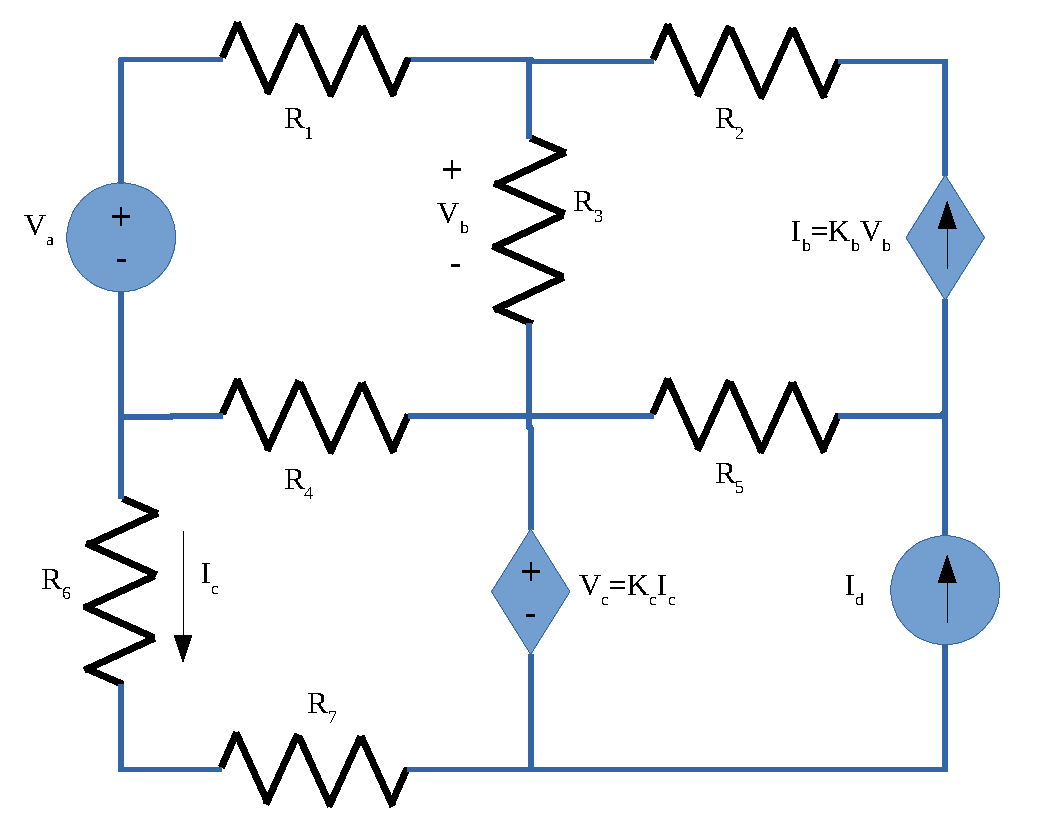
\includegraphics[width=1\linewidth]{circuit.pdf}
\caption{Circuit topography}
\label{fig:circuit}
\end{figure}

